\section{Results and discussion}
    \label{sec:results}

    \subsection{Latent Dirichlet allocation}

        Latent Dirichlet allocation was adjusted in our documents using five topics (components), the number of precedents we are considering. \autoref{fig:lda_topics} shows the top-20 words for each topic. From the barplot, we can see the following topics associated with the following BPs, justified by the following words:
        \begin{itemize}
                \item topic 1 \& BP 20: gratificação, inativos, atividade, desempenho, avaliação, gdata;
                \item topic 3 \& BP 4: salário, base, decisão, mínimo, constituição, cálculo;
                \item topic 4 \& BP 10: decisão, tribunal, constitucional, 10;
                \item topic 5 \& BP 14: acesso, direito, penal, inquérito, defeso, 14.
        \end{itemize}

        \begin{figure*}[!h]
                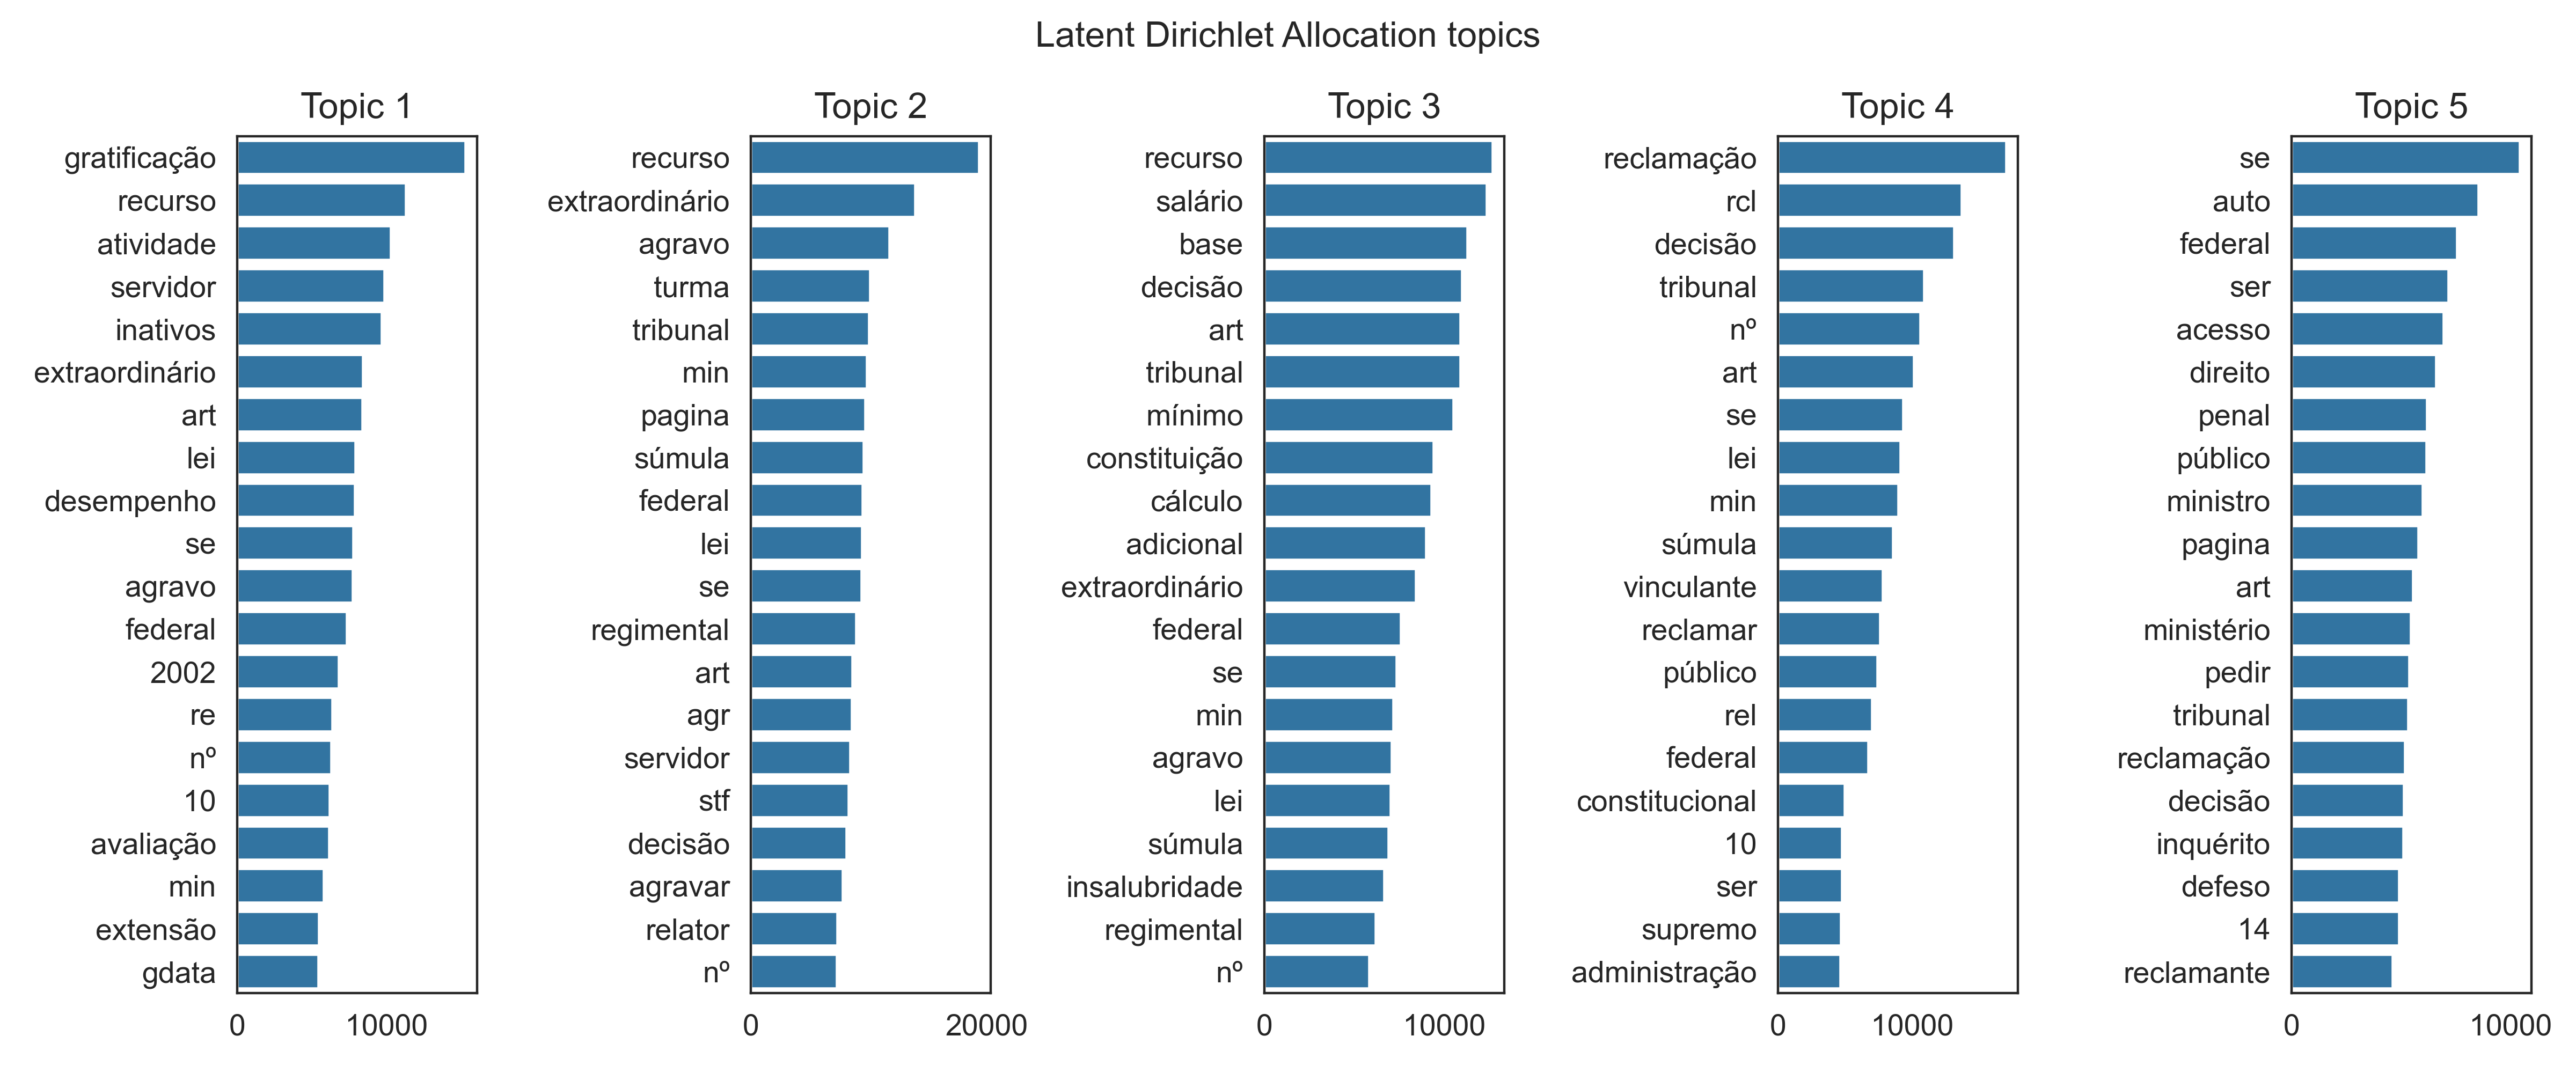
\includegraphics[width=\linewidth]{lda_topics.png}
                \caption{Top-20 words for each topic estimated with latent Dirichlet analysis.}
                \label{fig:lda_topics}
        \end{figure*}

        We can verify if the ``predicted'' topics match the real BPs being cited. Using this topic to BP assignment presented before, we get an accuracy of 0.76. That is, this topic modeling predicts the cited precedent correctly in 76\% of documents. We would expect 0.2 if it were a random assignment. So, LDA can extract the subjects of the BPs being cited.

    \subsection{Truncated SVD dimensionality reduction}

        \autoref{fig:svd_1} shows the resulting truncated SVD dimensionality reduction to 2. The color indicates the cited precedents, but the algorithm does not know that. We can see a pattern of data distribution, indicating that documents that cite the same BP are near each other.

        \begin{figure}[H]
                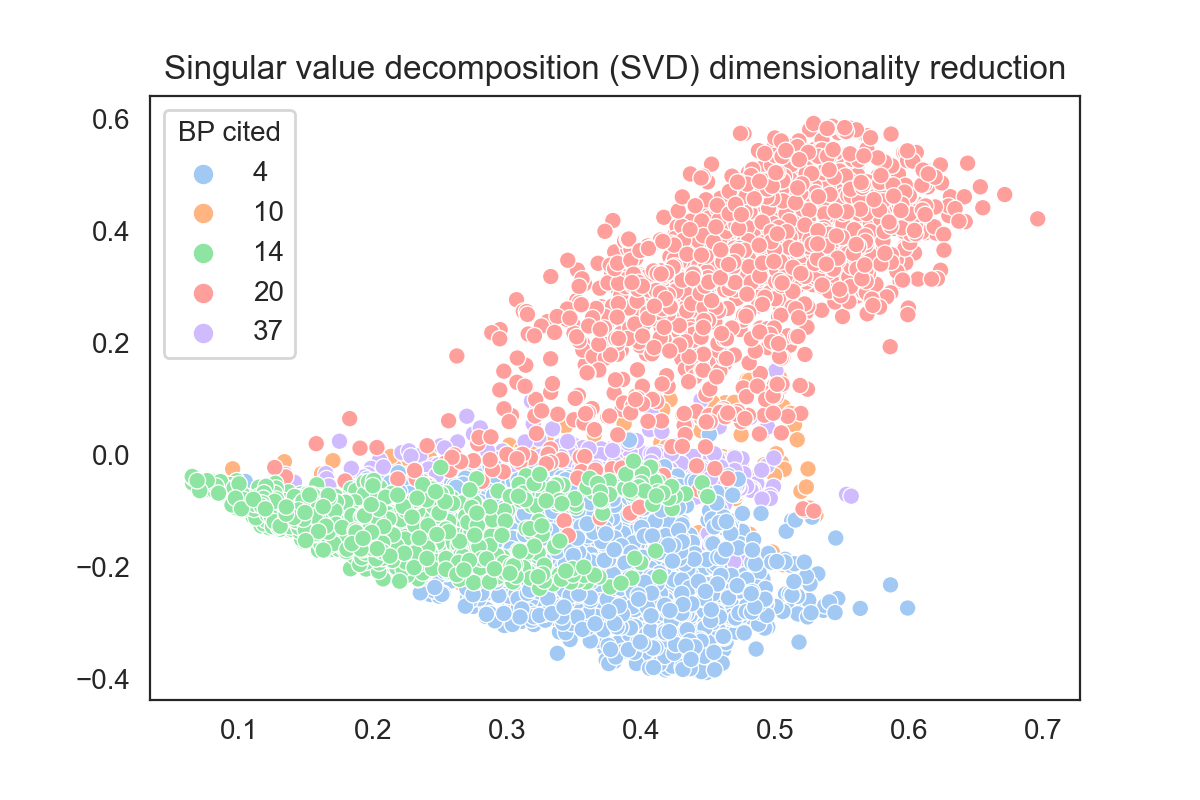
\includegraphics[width=\linewidth]{svd_1.png}
                \caption{Truncated singular value decomposition (SVD) dimensionality reduction to 2.}
                \label{fig:svd_1}
        \end{figure}

        \autoref{fig:svd_2_3}(a) and (b) present the result of dimensionality reduction to 3 dimensions. This graphic complements the last graphic, in the sense that it is more clear from this plot the fact that the documents can be separable in high dimensional space according to precedent citations.

        \begin{figure*}[!h]
                \centering
                \subfloat[\centering ]{{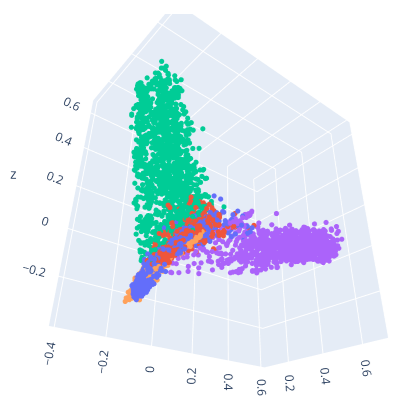
\includegraphics[width=0.4\linewidth]{svd_2.png} }}
                \qquad
                \subfloat[\centering ]{{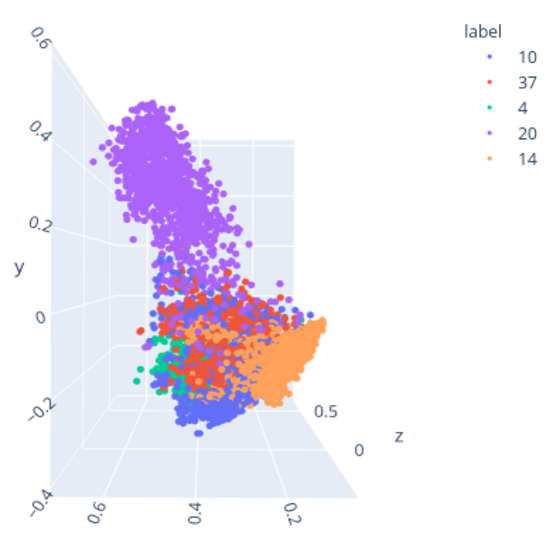
\includegraphics[width=0.4\linewidth]{svd_3.png} }}
                \caption{Truncated singular value decomposition (SVD) dimensionality reduction to 3.}
                \label{fig:svd_2_3}
        \end{figure*}

    \subsection{Linear regression}

        The results of classification using linear regression are presented in \autoref{tab:ridge}. Cross-validation to choose the Ridge regularization parameter was performed. All test metrics, i.e., precision, recall, and accuracy, are very high, which indicates the data is \textbf{linear separable}. \autoref{fig:rigde} shows the test confusion matrix, presenting how many documents from each BP were predicted as each BP. It is almost a diagonal matrix, indicating a very well-adjusted model.

        % Please add the following required packages to your document preamble:
        % \usepackage{multirow}
        \begin{table}[H]
                \centering
                \caption{Linear regression test metrics.}
                \label{tab:ridge}
                \begin{tabular}{c|cc|c}
                BP & Precision & Recall & Accuracy              \\ \hline
                4  & 0.96      & 0.91   & \multirow{5}{*}{0.95} \\
                10 & 0.94      & 0.93   &                       \\
                14 & 0.94      & 0.99   &                       \\
                20 & 0.99      & 0.95   &                       \\
                37 & 0.90      & 0.95   &                      
                \end{tabular}
        \end{table}

        \begin{figure}[H]
                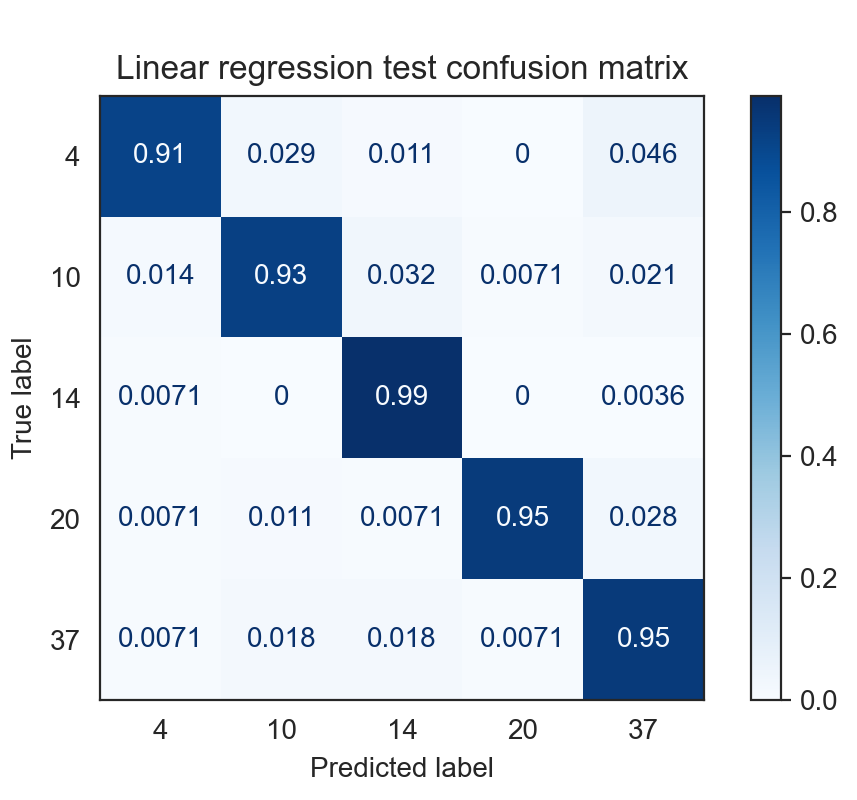
\includegraphics[width=\linewidth]{ridge.png}
                \caption{Linear regression test confusion matrix.}
                \label{fig:rigde}
        \end{figure}

    \subsection{Logistic regression}

        \autoref{tab:lr} presents the results of classification using logistic regression. Cross-validation to choose $C$ regularization parameter was performed. All test metrics, i.e., precision, recall, and accuracy, are very high. Comparing to linear regression, the accuracy is even higher. \autoref{fig:lr} (in \autoref{sec:confusion_matrices}, from now on) shows the test confusion matrix. It is also almost a diagonal matrix, indicating a very well-adjusted model.

        % Please add the following required packages to your document preamble:
        % \usepackage{multirow}
        \begin{table}[H]
                \centering
                \caption{Logistic regression test metrics.}
                \label{tab:lr}
                \begin{tabular}{c|cc|c}
                BP & Precision & Recall & Accuracy              \\ \hline
                4  & 0.98      & 0.97   & \multirow{5}{*}{0.97} \\
                10 & 0.96      & 0.96   &                       \\
                14 & 0.98      & 0.99   &                       \\
                20 & 0.97      & 0.97   &                       \\
                37 & 0.95      & 0.96   &                      
                \end{tabular}
        \end{table}

    \subsection{Linear discriminant analysis}

        The results of classification using linear discriminant analysis are presented in \autoref{tab:lda}. All test metrics, i.e., precision, recall, and accuracy, are very high, which indicates the data is \textbf{linearly separable}. \autoref{fig:lda} shows the test confusion matrix, almost a diagonal matrix.

        % Please add the following required packages to your document preamble:
        % \usepackage{multirow}
        \begin{table}[H]
                \centering
                \caption{Linear discriminant analysis test metrics.}
                \label{tab:lda}
                \begin{tabular}{c|cc|c}
                BP & Precision & Recall & Accuracy              \\ \hline
                4  & 0.97      & 0.91   & \multirow{5}{*}{0.95} \\
                10 & 0.91      & 0.95   &                       \\
                14 & 0.97      & 0.99   &                       \\
                20 & 0.99      & 0.93   &                       \\
                37 & 0.90      & 0.96   &                      
                \end{tabular}
        \end{table}

    \subsection{K-nearest neighbors}

        \autoref{tab:k_nn} presents the results of using k-nearest neighbors for classification. For choosing the number $k$ of neighbors, it was performed cross-validation, and the chosen hyperparameter was $k = 1$. Test metrics, i.e., precision, recall, and accuracy, are high. \autoref{fig:k_nn} shows the test confusion matrix, which indicates high performance.
        
        % Please add the following required packages to your document preamble:
        % \usepackage{multirow}
        \begin{table}[H]
                \centering
                \caption{K-nearest neighbors test metrics.}
                \label{tab:k_nn}
                \begin{tabular}{c|cc|c}
                BP & Precision & Recall & Accuracy              \\ \hline
                4  & 0.93      & 0.95   & \multirow{5}{*}{0.93} \\
                10 & 0.87      & 0.90   &                       \\
                14 & 0.95      & 0.96   &                       \\
                20 & 0.97      & 0.95   &                       \\
                37 & 0.92      & 0.90   &                      
                \end{tabular}
        \end{table}

    \subsection{Random forest}

        The results of using a random forest for classification are shown in \autoref{tab:rf}. Hyperparameters of maximum tree depth and the number of estimators were chosen using cross-validation, resulting in no maximum depth and number of trees equal to 100. From test metrics, we see a very high performance. The test confusion matrix is also excellent, almost a diagonal matrix (\autoref{fig:rf}).
        
        % Please add the following required packages to your document preamble:
        % \usepackage{multirow}
        \begin{table}[H]
                \centering
                \caption{Random forest test metrics.}
                \label{tab:rf}
                \begin{tabular}{c|cc|c}
                BP & Precision & Recall & Accuracy              \\ \hline
                4  & 0.98      & 0.96   & \multirow{5}{*}{0.96} \\
                10 & 0.91      & 0.95   &                       \\
                14 & 0.98      & 0.99   &                       \\
                20 & 0.98      & 0.96   &                       \\
                37 & 0.94      & 0.93   &                      
                \end{tabular}
        \end{table}

    \subsection{Support vector machine}

        Test metrics relative to the support vector machine used for classification are presented in \autoref{tab:svm}. From the metrics, we see very high performance in test data. The hyperparameters, which include kernel function (linear vs. RBF), regularization parameter $C$, and $\gamma$, were chosen by CV, and the result was $C = 100$, $\gamma = 0.001$, and kernel RBF. The test confusion matrix is excellent, which indicates a very high model performance (\autoref{fig:svm}).
        
        % Please add the following required packages to your document preamble:
        % \usepackage{multirow}
        \begin{table}[H]
                \centering
                \caption{Support vector machine test metrics.}
                \label{tab:svm}
                \begin{tabular}{c|cc|c}
                BP & Precision & Recall & Accuracy              \\ \hline
                4  & 0.99      & 0.97   & \multirow{5}{*}{0.97} \\
                10 & 0.95      & 0.97   &                       \\
                14 & 0.98      & 0.99   &                       \\
                20 & 0.98      & 0.97   &                       \\
                37 & 0.96      & 0.96   &                      
                \end{tabular}
        \end{table}

    \subsection{Further discussion}

        It is clear from the experiments that our dataset is separable, in the sense of being able to be separated according to the Binding Precedent citation. Even more, the data seems to be \textbf{linearly separable}, as indicated by linear regression, logistic regression, and linear discriminant analysis. One very interesting property is that the documents, in very high dimensional space, are closer if they cite the same precedent, which is indicated by the results of truncated SVD dimensionality reduction and k-NN.

        Using latent Dirichlet allocation, and analyzing the results, we could verify that the topics, in general, extracted words and the subject, in general, of the cited precedents. We saw that, with five BPs and five topics, each topic could be associated with a BP, and the accuracy of this association was surprisingly high, over 0.75, against 0.2, the accuracy of a random assignment.

        With these models in hand, one could expand these experiments, considering more documents, more precedents, more sophisticated models, and build a model that confidently predicts the precedent being cited.

